\section{ Dataset }
We crawled vine for over a month and did a snowball sampling to collect over 12000 videos which were ranked to be popular by the vine service over 2 weeks in december. We collected an additional 20,000 videos which were not classified as popular. The popularity distribution of the whole dataset follows as expected a zipf distribution. The videos were then passed through a sampling process, where we sampled one frame from each second of the video lenght. The sampling was chosen purely hurestically. The main aim behind the sampling was to measure the perceptual sentiment as the video progresses. The figure \ref{fig:CDF_posts} shows the distribution of the crawled vine posts. The popularity distribution follows a long tail pattern, which is a expected behaviour among a socially influenced dataset.
\par
For training of the Visual sentiment detector, we use the 1 million annotated flicker images opened up to the community by the Sentibank researchers. The accuracy of detector was measured over this training dataset and we baseline our detector's performance based on the mean probability confidence of the detector for the training dataset. 

\begin{figure}
\centering
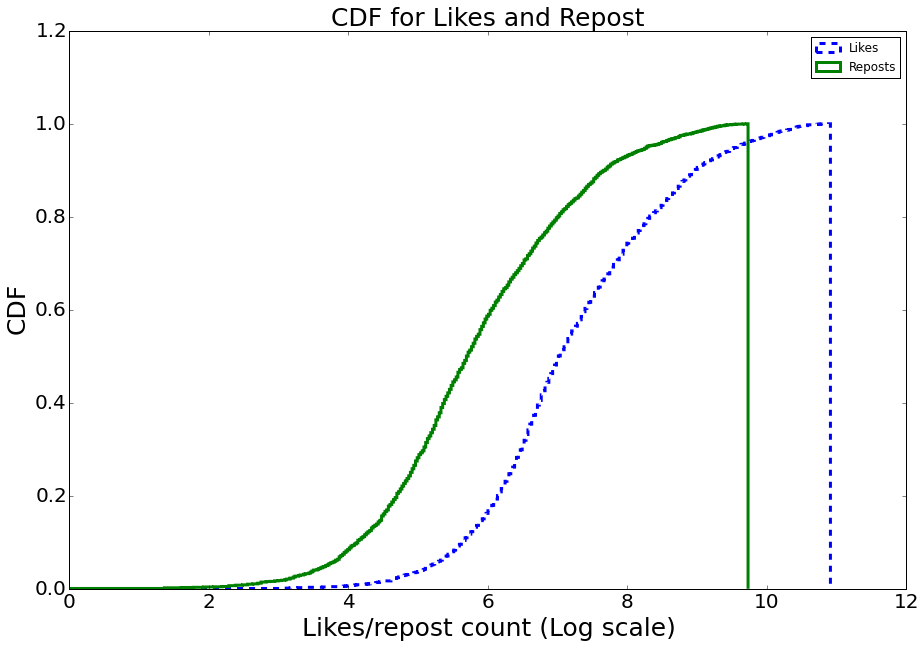
\includegraphics[width=\columnwidth]{plots/CDF_Like_reposts}
\caption{\textsl{ CDF of Like count and Repost count.}}
\label{fig:CDF_posts}
\end{figure}